\documentclass[a4paper,11pt]{article}
\usepackage{amsmath,bm}
\usepackage{amssymb}
\usepackage{color}
\usepackage{tikz}
\usepackage{colortbl}

\begin{document}

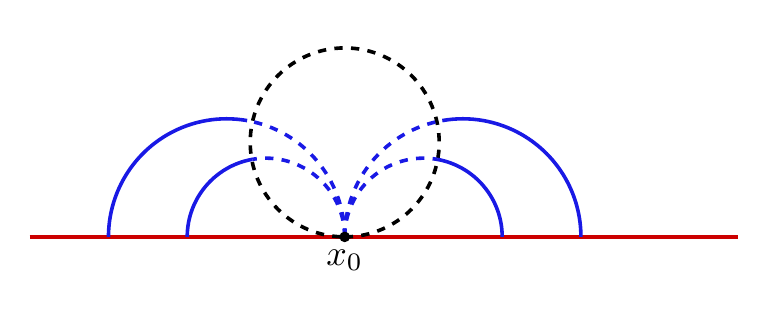
\begin{tikzpicture}
	\draw[color=red!80!black,line width=1.5pt] (-5,0)--(4,0);
	\draw[color=black,dashed,line width=1.3pt] (-1,0) arc(-90:270:1.2) node[pos=0.5,above,sloped]{$\textcolor{black}{}$};
	\draw[color=blue!90!yellow,line width=1.3pt] (1,0) arc(0:80:1) node[pos=0.5,above,sloped]{$\textcolor{black}{}$};
	\draw[color=blue!90!yellow,dashed,line width=1.3pt] (-1,0) arc(180:80:1) node[pos=0.5,above,sloped]{$\textcolor{black}{}$}; 
	\draw[color=blue!90!yellow,line width=1.3pt] (2,0) arc(0:100:1.5);
	\draw[color=blue!90!yellow,dashed,line width=1.3pt] (-1,0) arc(180:100:1.5);      
	\draw[color=blue!90!yellow,line width=1.3pt] (-3,0) arc(180:100:1);
	\draw[color=blue!90!yellow,dashed,line width=1.3pt] (-1,0) arc(0:100:1);  
	\draw[color=blue!90!yellow,line width=1.3pt] (-4,0) arc(180:80:1.5);
	\draw[color=blue!90!yellow,dashed,line width=1.3pt] (-1,0) arc(0:80:1.5);  
	\draw[fill](-1,0)circle(0.06)node[below,scale=1.3]{$ x_0 $};
\end{tikzpicture}

\end{document}